\documentclass[11pt,aspectratio=169]{beamer}

\usetheme{Madrid}
\usecolortheme{default}
\setbeamertemplate{navigation symbols}{}
\setbeamertemplate{footline}[frame number]

\usepackage{graphicx}
\usepackage{booktabs}
\usepackage{amsmath}
\usepackage{array}
\usepackage{ragged2e}

\graphicspath{{outputs/plots/}}

\definecolor{hopeblue}{RGB}{17,84,124}
\definecolor{hopeteal}{RGB}{25,133,115}
\definecolor{hopegold}{RGB}{203,126,41}
\definecolor{softbg}{RGB}{245,248,250}
\definecolor{softline}{RGB}{220,228,234}

\setbeamercolor{structure}{fg=hopeblue}
\setbeamercolor{title}{fg=hopeblue}
\setbeamercolor{frametitle}{fg=hopeblue,bg=softbg}
\setbeamercolor{block title}{fg=white,bg=hopeblue}
\setbeamercolor{block body}{fg=black,bg=softbg}
\setbeamercolor{block title alerted}{fg=white,bg=hopegold}
\setbeamercolor{block body alerted}{fg=black,bg=softbg}
\setbeamercolor{block title example}{fg=white,bg=hopeteal}
\setbeamercolor{block body example}{fg=black,bg=softbg}
\setbeamerfont{frametitle}{size=\Large,series=\bfseries}
\setbeamerfont{title}{size=\Large,series=\bfseries}
\setbeamerfont{normal text}{size=\normalsize}

\newcommand{\statcard}[2]{%
  \begin{beamercolorbox}[wd=\linewidth,rounded=true,sep=0.8em]{block body}
    {\Large\textbf{#1}}\\[0.2em]
    #2
  \end{beamercolorbox}
}

\title{IDSC 2026 Pitch Deck}
\subtitle{Team VZ}
\author{Izzar Suly Nashrudin and Risma Muslimah}
\date{}
\titlegraphic{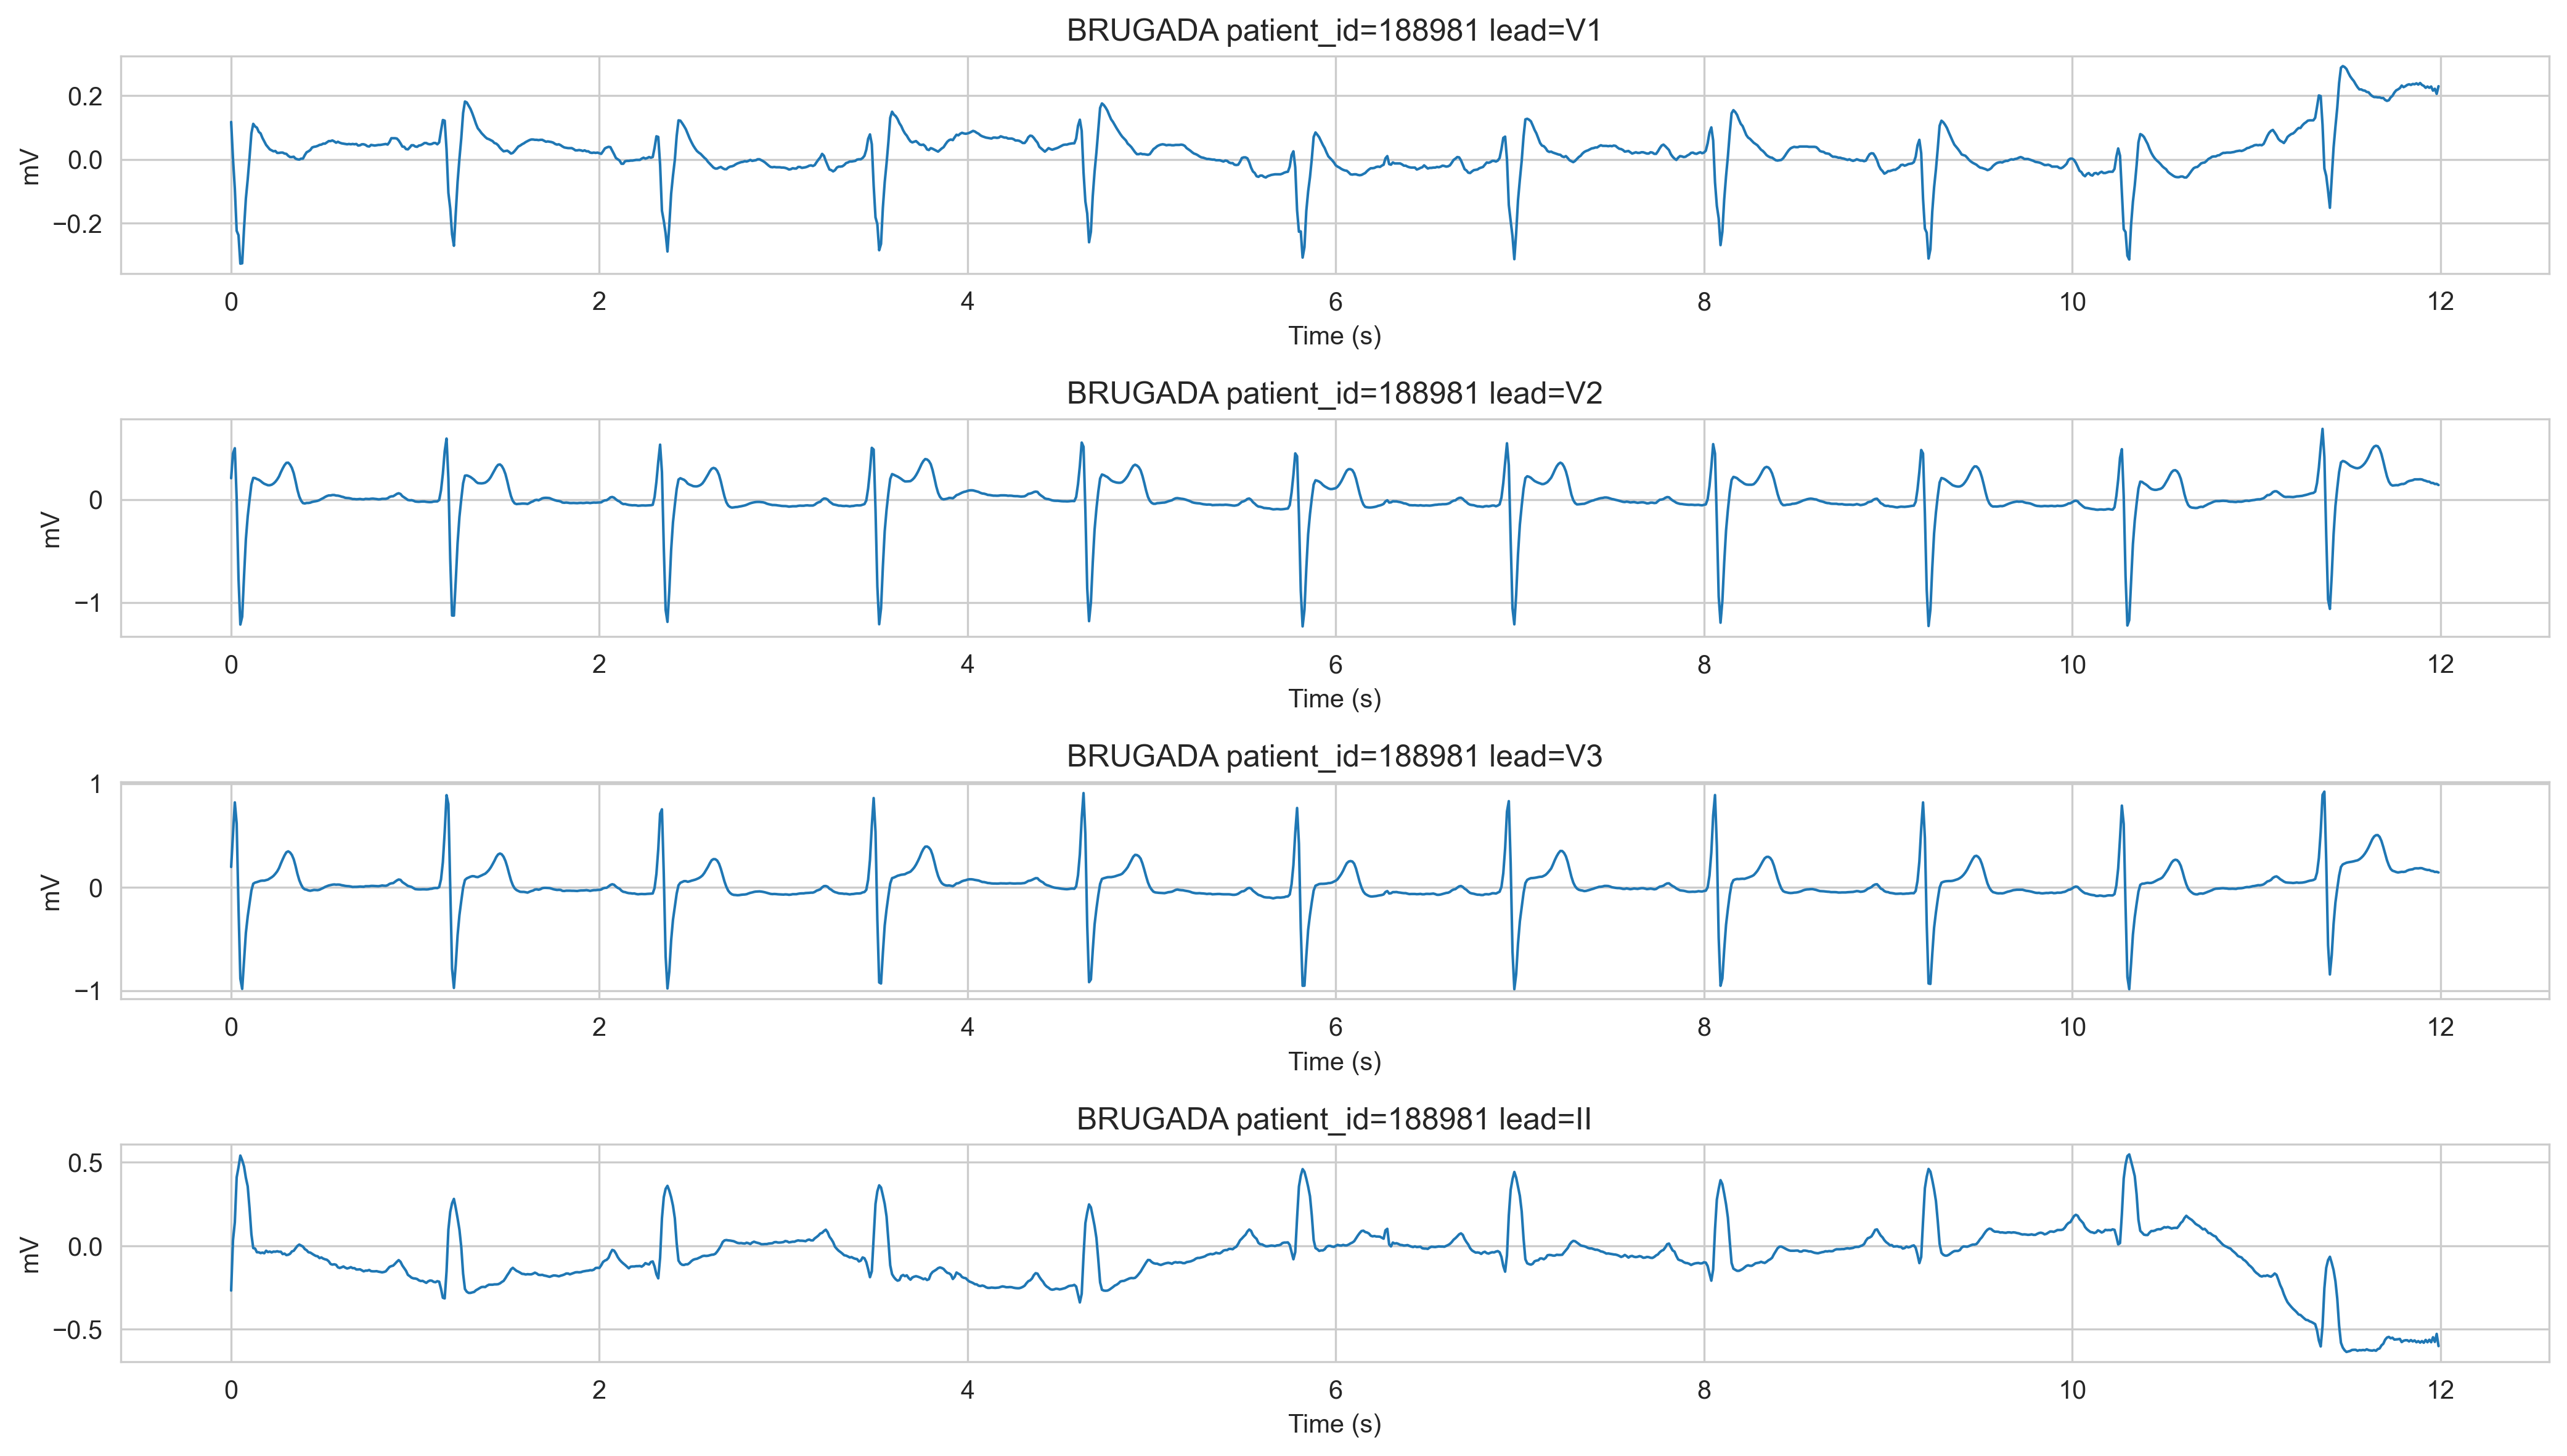
\includegraphics[width=0.25\linewidth]{EDA Brugada 188981 Selected Leads.png}}

\begin{document}

% Suggested speaking time: 0:00--0:20
\begin{frame}[plain]
  \centering
  {\Huge\bfseries IDSC 2026 Pitch Deck\par}
  \vspace{0.6em}
  {\Large\bfseries Helping clinicians miss fewer Brugada cases\par}
  \vspace{0.5em}
  {\large Team VZ: Izzar Suly Nashrudin and Risma Muslimah\par}
  \vspace{1em}
  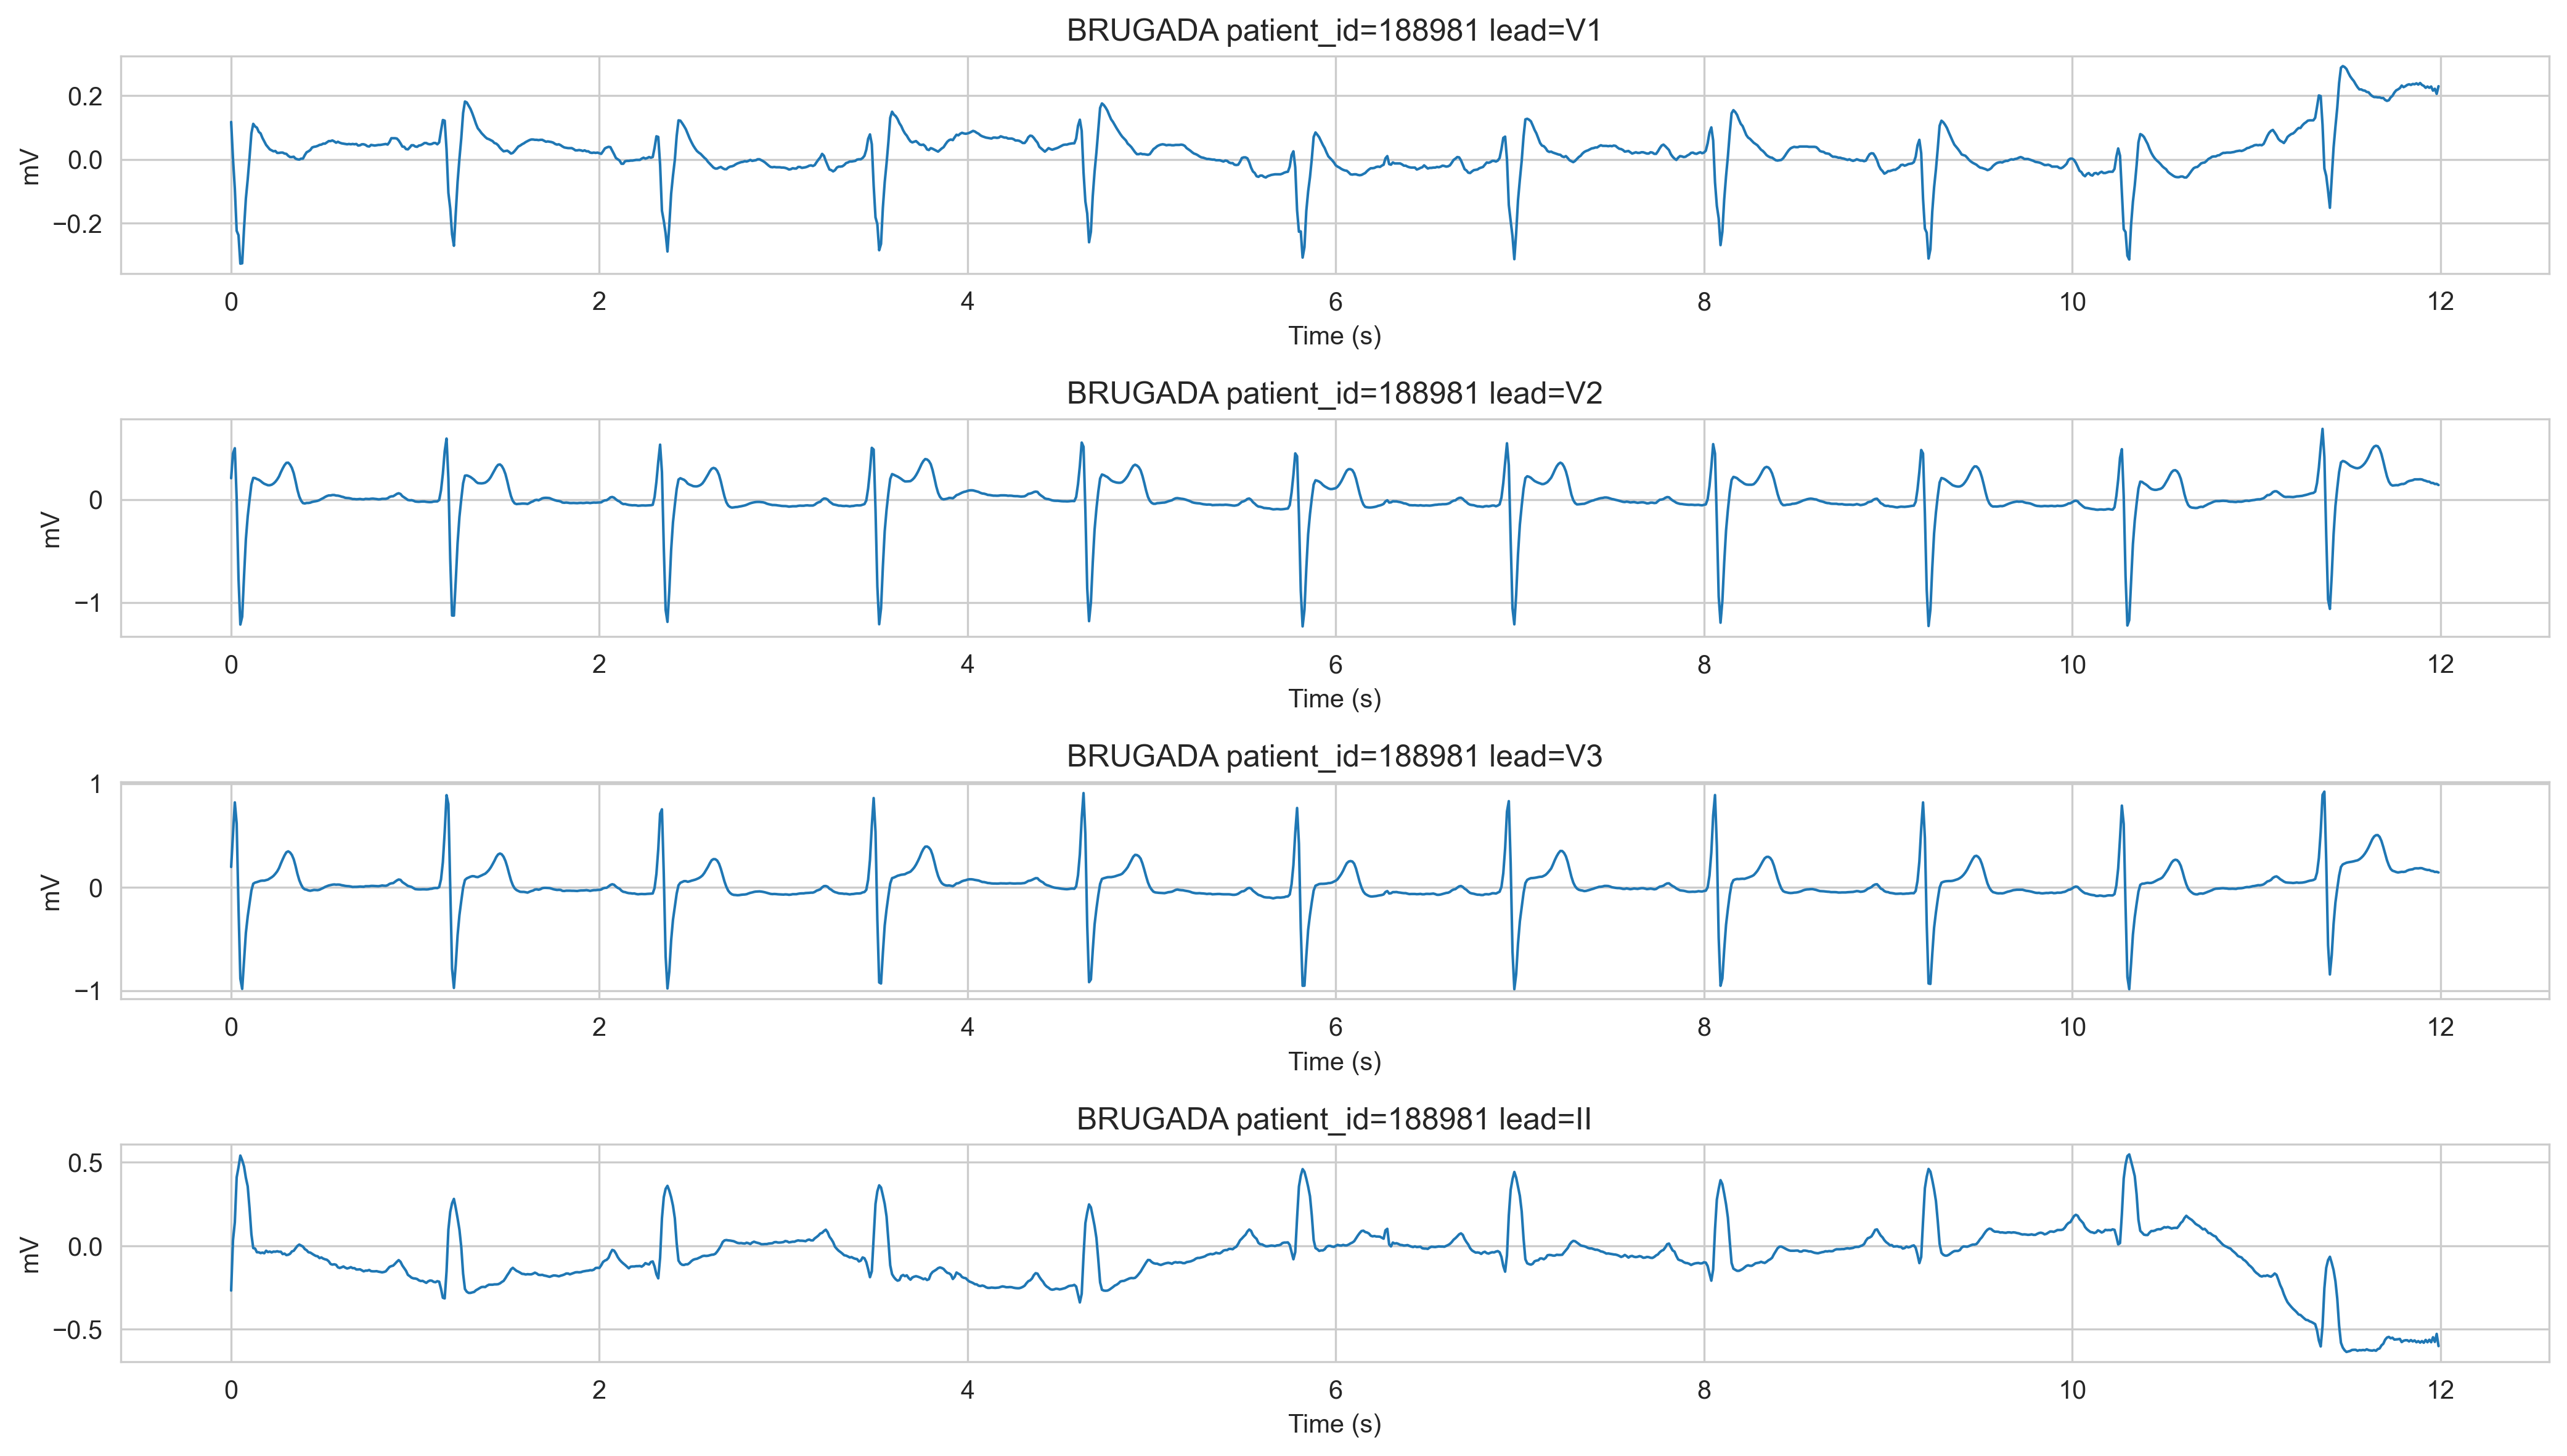
\includegraphics[width=0.26\linewidth]{EDA Brugada 188981 Selected Leads.png}
  \vspace{0.8em}
  \par
  \normalsize
  A safety-aware ECG benchmark for earlier review of high-risk patients.
\end{frame}

% Suggested speaking time: 0:20--0:50
\begin{frame}[t]{One missed Brugada ECG can be fatal}
\begin{columns}[T,onlytextwidth]
\column{0.58\textwidth}
\justifying
\begin{block}{Why judges should care}
\begin{itemize}
  \item Brugada syndrome can lead to sudden cardiac death.
  \item In screening, missing a true case matters more than one extra review.
  \item So the key question is: ``Who are we still missing?''
\end{itemize}
\end{block}

\begin{alertblock}{Our story}
We use ordinary 12-lead ECGs to build a screening aid designed to miss fewer dangerous patients.
\end{alertblock}

\column{0.38\textwidth}
\statcard{356}{patients in the main ECG cohort}
\vspace{0.3em}
\statcard{69}{Brugada cases in the full benchmark}
\vspace{0.3em}
\statcard{11}{models on the same ECG-only split}
\end{columns}
\end{frame}

% Suggested speaking time: 0:50--1:25
\begin{frame}[t]{We benchmarked for safety, not just score}
\begin{columns}[T,onlytextwidth]
\column{0.55\textwidth}
\begin{block}{What we did}
\begin{itemize}
  \item Read raw 12-lead ECGs.
  \item Compare 11 models on one shared patient split.
  \item Keep the main benchmark ECG-only.
\end{itemize}
\end{block}

\begin{exampleblock}{Clinical design choice}
Metadata stays in a separate ablation, so the main result is driven by the ECG itself.
\end{exampleblock}

\column{0.42\textwidth}
\begin{block}{How we judged models}
\begin{itemize}
  \item Strong overall performance still matters.
  \item But missing risky patients matters more.
  \item Consistency and practicality break ties.
\end{itemize}
\end{block}

\begin{alertblock}{Key message}
We do not let a high score hide dangerous false negatives.
\end{alertblock}
\end{columns}
\end{frame}

% Suggested speaking time: 1:25--1:50
\begin{frame}[t]{We did not bet on one lucky algorithm}
\begin{columns}[T,onlytextwidth]
\column{0.48\textwidth}
\begin{block}{Three model families}
\begin{itemize}
  \item \textbf{Feature models}: XGBoost, Random Forest, SVM-RBF, and AdaBoost.
  \item \textbf{Deep sequence models}: CNN, ResNet-1D, CNN+BiGRU, and Transformer Encoder.
  \item \textbf{Representation learning}: transfer learning, VICReg, and Echo State Network.
\end{itemize}
\end{block}

\column{0.48\textwidth}
\begin{alertblock}{Why this matters}
\begin{itemize}
  \item Each family reads the ECG differently.
  \item All 11 models use the same split, so the comparison is fair.
  \item If one model still wins, the recommendation is easier to trust.
\end{itemize}
\end{alertblock}

\begin{beamercolorbox}[wd=\linewidth,rounded=true,sep=0.8em]{block body}
\textbf{Takeaway:} we tested breadth, then chose the model that balances performance with screening safety.
\end{beamercolorbox}
\end{columns}
\end{frame}

% Suggested speaking time: 1:50--2:20
\begin{frame}[t]{One model won on safety and performance}
\begin{columns}[T,onlytextwidth]
\column{0.48\textwidth}
\begin{exampleblock}{Recommended model}
\textbf{Transfer learning model}
\begin{itemize}
  \item \textbf{Headline metric:} PR-AUC 0.676
  \item \textbf{Clinical takeaway:} only 5 false negatives
\end{itemize}
\end{exampleblock}

\begin{alertblock}{The story in one sentence}
The best leaderboard model and safest screening model can differ. Here, they converge on the same transfer model.
\end{alertblock}

\column{0.48\textwidth}
\begin{block}{Why this result matters}
\justifying
This is what we want in healthcare: a model that performs strongly overall while still reducing the number of missed risky patients.
\end{block}

\vspace{0.3em}
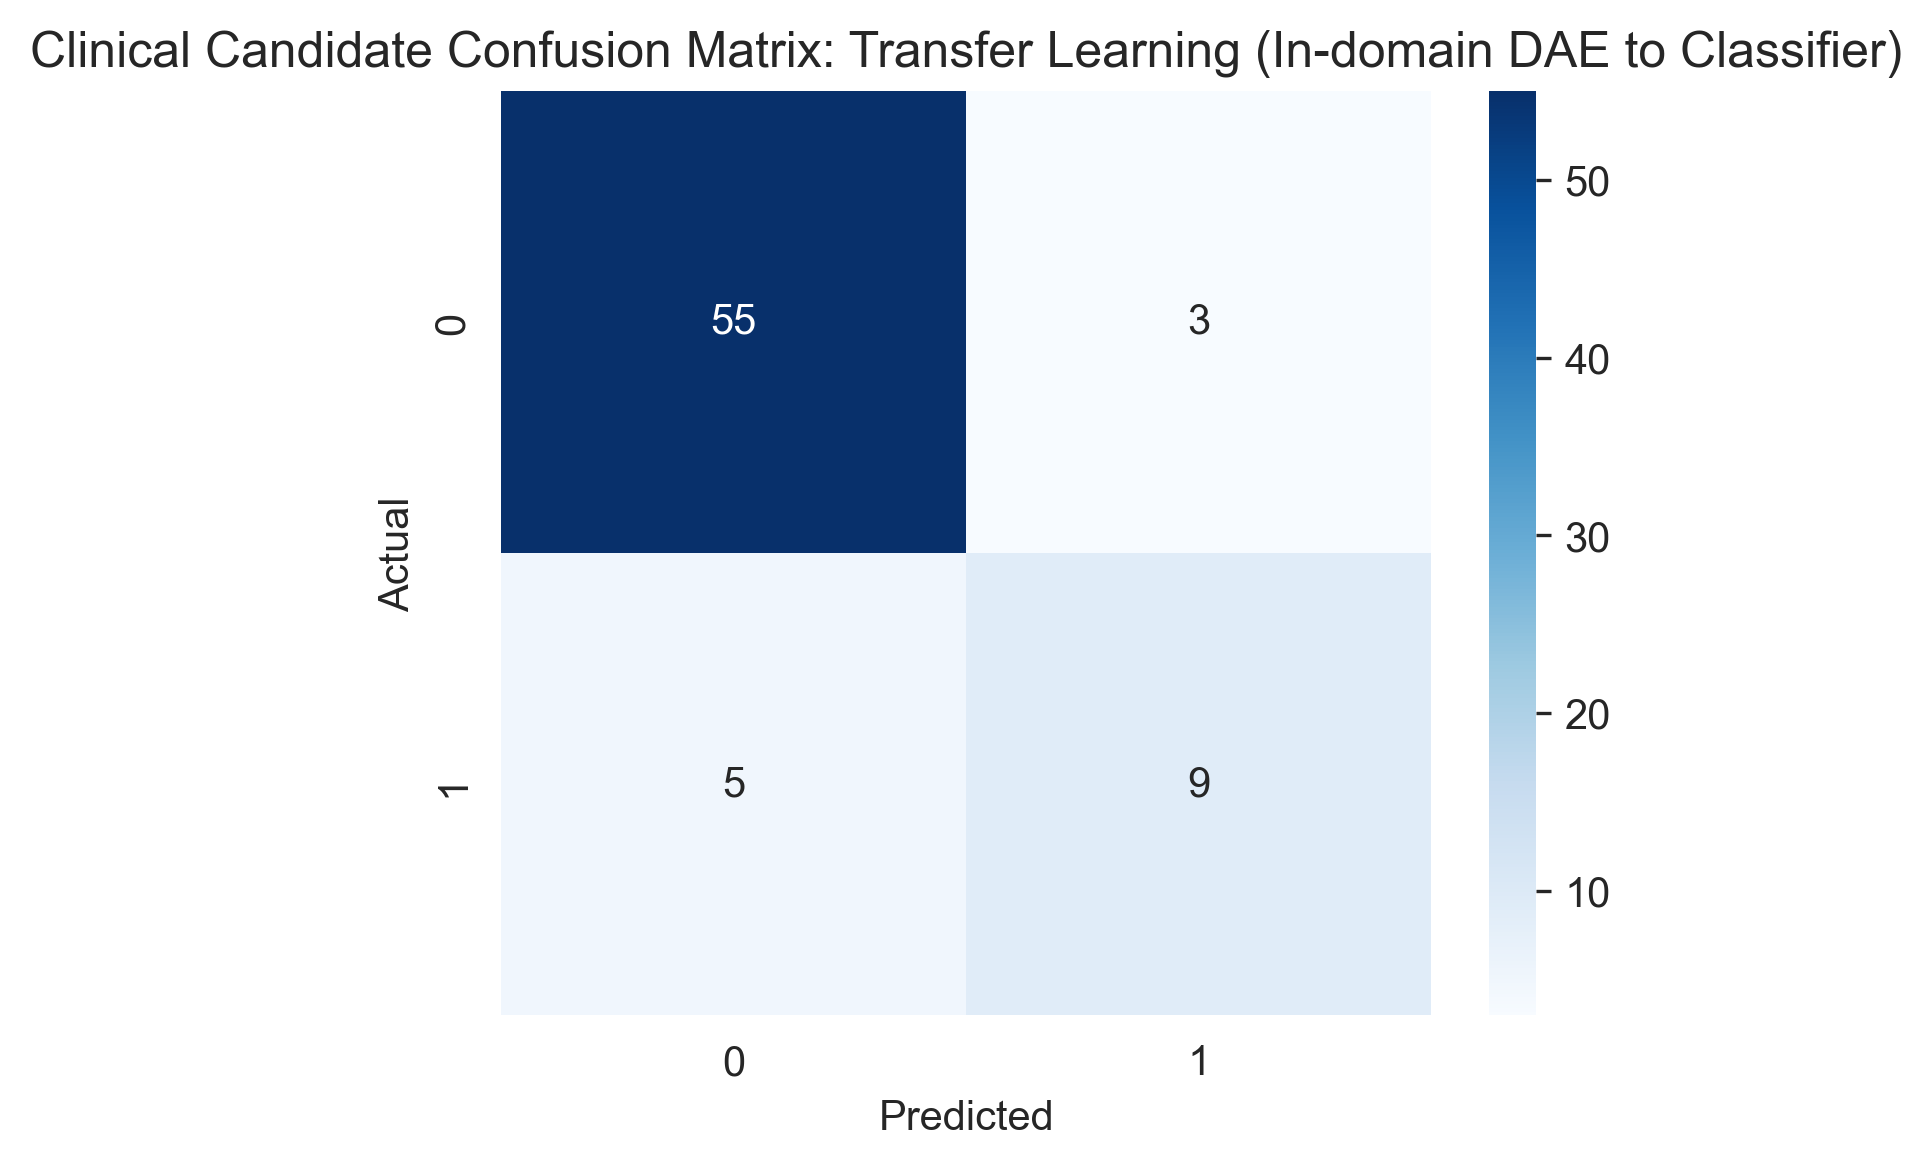
\includegraphics[width=\linewidth,height=0.36\textheight,keepaspectratio]{Validation Clinical Candidate Confusion Matrix.png}
\end{columns}
\end{frame}

% Suggested speaking time: 2:20--2:45
\begin{frame}[t]{It fits the way clinicians already work}
\begin{columns}[T,onlytextwidth]
\column{0.54\textwidth}
\begin{block}{Why it is practical}
\begin{itemize}
  \item It uses standard 12-lead ECGs already available in care settings.
  \item It works as a second reader for earlier specialist attention.
  \item It still highlights plausible precordial regions.
\end{itemize}
\end{block}

\begin{exampleblock}{Why it is clinically honest}
\begin{itemize}
  \item We explicitly surface false negatives.
  \item We separate aggregate performance from safety decisions.
  \item We frame it as a second reader, not autonomous diagnosis.
\end{itemize}
\end{exampleblock}

\column{0.42\textwidth}
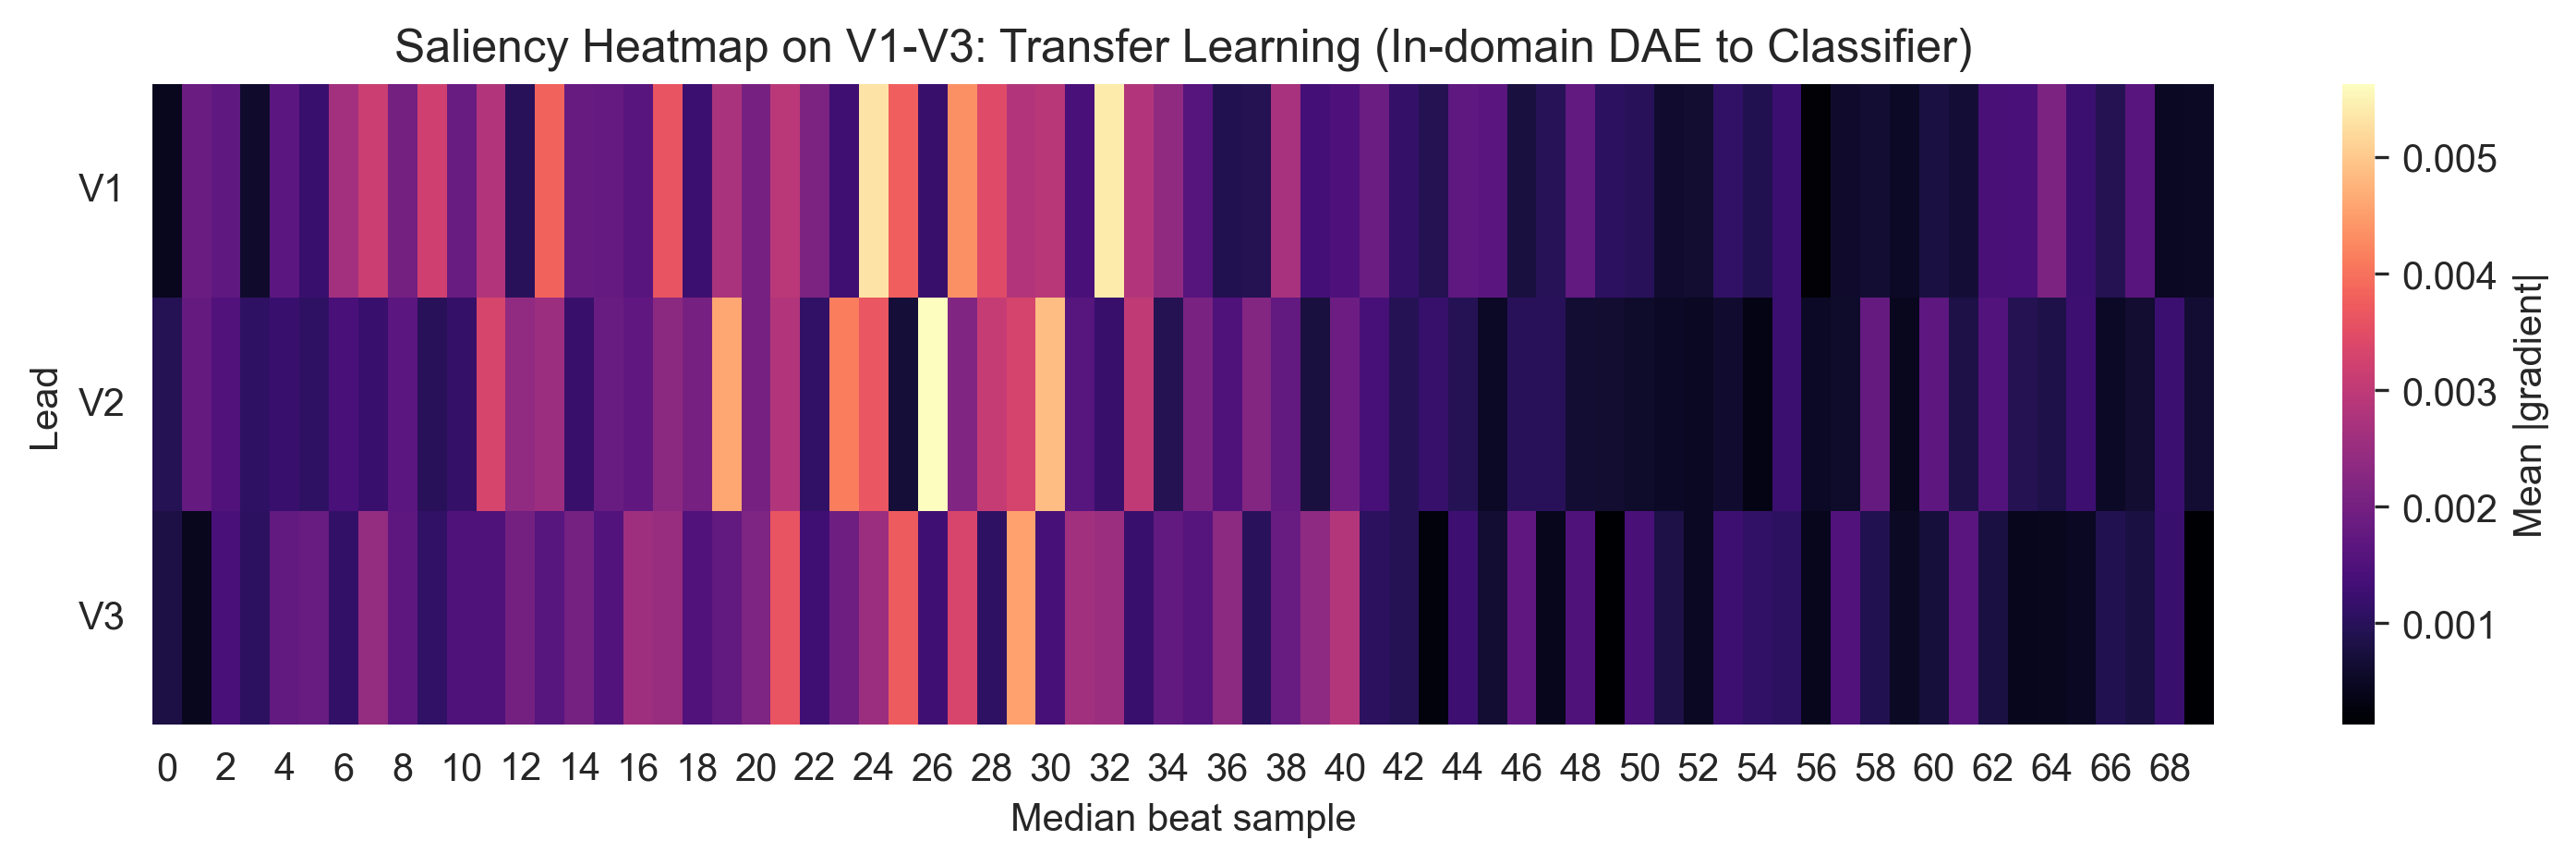
\includegraphics[width=\linewidth,height=0.25\textheight,keepaspectratio]{Interpretability Sequence V1 V3 Saliency Heatmap.png}

\vspace{0.3em}
\begin{beamercolorbox}[wd=\linewidth,rounded=true,sep=0.3em]{block body}
\centering
\textbf{Simple value:} help clinicians notice risky ECGs earlier.
\end{beamercolorbox}
\end{columns}
\end{frame}

% Suggested speaking time: 2:45--3:00
\begin{frame}[t]{From ordinary ECGs to earlier action}
\begin{block}{What we achieved}
We built a safety-aware ECG benchmarking pipeline that turns raw 12-lead signals into a practical Brugada screening aid.
\end{block}

\begin{columns}[T,onlytextwidth]
\column{0.48\textwidth}
\begin{exampleblock}{Near-term value}
\begin{itemize}
  \item Triage support
  \item Second-reader assistance
  \item Better prioritization for specialist review
\end{itemize}
\end{exampleblock}

\column{0.48\textwidth}
\begin{alertblock}{Next step}
\begin{itemize}
  \item External validation
  \item Prospective threshold calibration
  \item Real clinical workflow integration
\end{itemize}
\end{alertblock}
\end{columns}

\vspace{0.6em}
\centering
\Large\textbf{Miss fewer risky patients. Review them earlier.}\\[0.2em]
\large That is the kind of impact AI should bring to healthcare.\\[0.6em]
\scriptsize Project repository: \url{https://github.com/avezoor/IDSC2026}
\end{frame}

\end{document}
